\section{Creating image of 3 channels}

The three gray scale images are created in Matlab as simple matrices containing zeros and ones. These matrices are then concatenated along the third dimension to form the three color channels of the RGB image. See figure \ref{fig:task1}.

\begin{figure}[!hbt]
  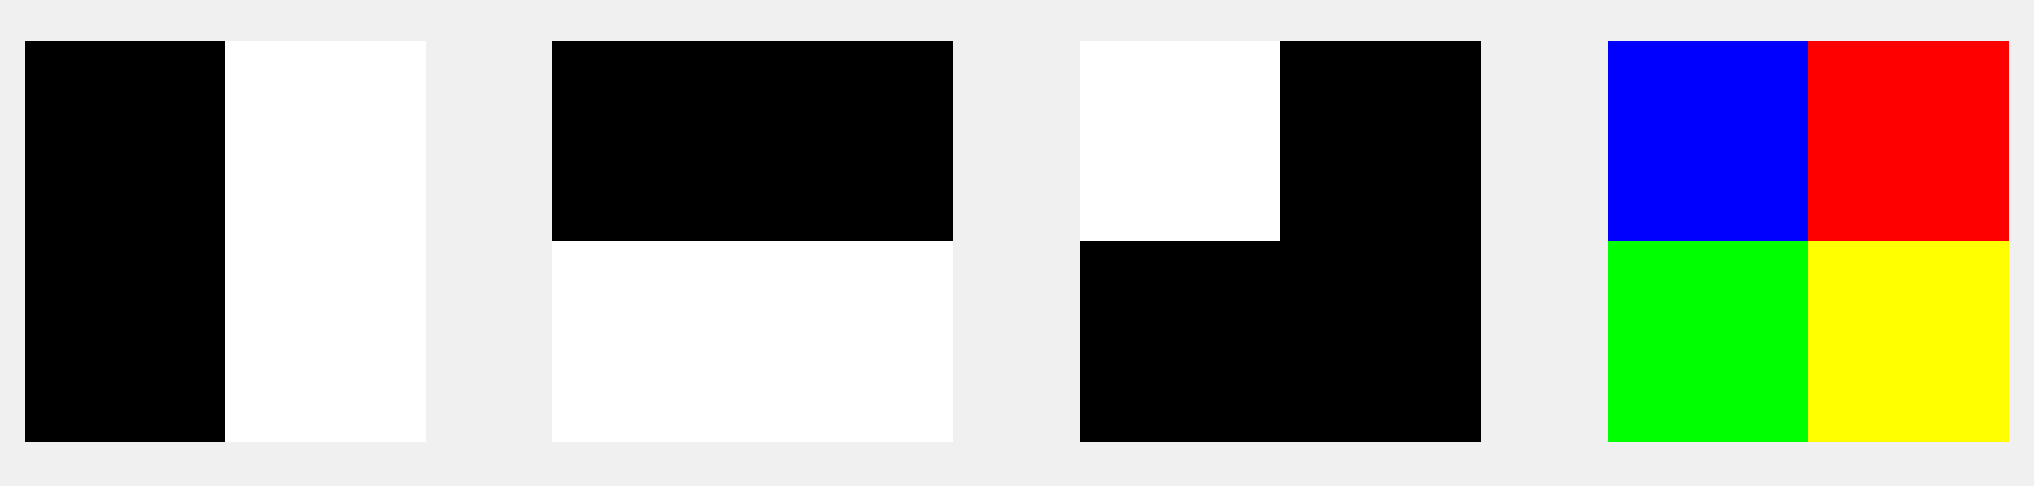
\includegraphics[width=\textwidth]{./img/task1.png}
  \caption{Results of Exercise 1}
  \label{fig:task1}
\end{figure}
